\section{Pointer und Arrays \verweis{6}}
	\begin{minipage}[t]{7 cm}
		\subsection{Arbeisspeicher - Memory Map \verweis{6.1}}
			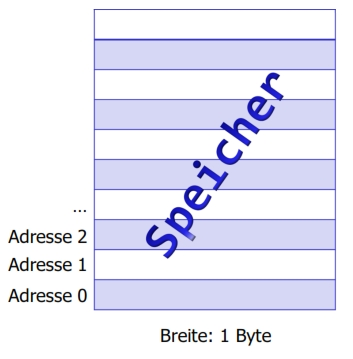
\includegraphics[width=0.9\textwidth]{pics/arbeitsspeicher.jpg}
			
			\begin{compactitem}
				\item Der gesamte Speicher besteht aus einer Folge von einzelnen Bytes, welche durchnumeriert werden.
				\item Diese eindeutige Nummer einer Speicherzelle wird als Adresse bezeichnet.
				\item Bei einem byteweise adressierbaren Speicher (ist üblich) liegt an jeder Adresse genau 1 Byte.
			\end{compactitem}
	\end{minipage}
	\hspace*{0.5cm}
	\begin{minipage}[t]{10.5 cm}
		\subsection{Pointer \verweis{6.1}}
			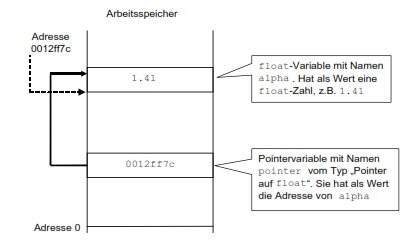
\includegraphics[width=1\textwidth]{pics/pointer.jpg}
				
			\begin{compactitem}
				\item Ein Pointer ist eine Variable, welche die Adresse einer im Speicher befindlichen Variablen oder Funktion aufnehmen kann.
				\item Man sagt, der Pointer zeige (to point) auf diese Speicherzelle.
				\item Pointer in C sind typisiert, sie zeigen auf eine Variable des definierten Typs.
				\item Der Speicherbereich, auf den ein bestimmter Pointer zeigt, wird entsprechend des definierten Pointer-Typs interpretiert.
				\item Der Speicherbedarf einer Pointervariablen ist unabhängig vom Pointer-Typ. Er ist so gross, dass die maximale Adresse Platz findet (z.B. 32 Bit).
			\end{compactitem}
	\end{minipage}	

	\begin{minipage}[t]{10 cm}
		\subsubsection{Definition einer Pointervariablen \verweis {6.1}}		
			\vspace*{-0.3cm}\lstinputlisting[language=C,tabsize=2]{code/pointer_init.c}
	\end{minipage}
	\hspace*{0.5cm}
	\begin{minipage}[t]{8.5 cm}
		\subsubsection{Initialisierung mit Nullpointer \verweis {6.1}}
			NULL ist vordefiniert (in $stddef.h$) und setzt den Pointer auf einen definierten Nullwert. Besser ist es, statt NULL direkt 0 zu verwenden.
			\vspace*{-0.2cm}\lstinputlisting[language=C,tabsize=2]{code/pointer_null.c}
	\end{minipage}		
			
	\begin{minipage}[t]{9 cm}
		\subsubsection{Der Adressoperator (Referenzierung) \verweis {6.1}}	
			Ist $x$ eine Variable vom Typ $Typname$, so liefert der	Ausdruck $\&x$ einen Pointer auf die Variable $x$, d.h. er liefert die Adresse der Variablen $x$.	
			\lstinputlisting[language=C,tabsize=2]{code/pointer_adressoperator.c}
	\end{minipage}
	\hspace*{0.5cm}
	\begin{minipage}[t]{9 cm}
		\subsubsection{Der Inhaltsoperator * (Dereferenzierung) \verweis {6.1}}
			Ist $ptr$ ein Pointer vom Typ $Typname$, so liefert der	Ausdruck $*ptr$ den Inhalt der Speicherzelle, auf welche $ptr$ zeigt.
			\vspace*{-0.2cm}\lstinputlisting[language=C,tabsize=2]{code/pointer_inhaltsoperator.c}
	\end{minipage}	
	
	\subsubsection{Beispiele Darstellung in graphischer Pointernotation}		
		\begin{minipage}[t]{6 cm}
			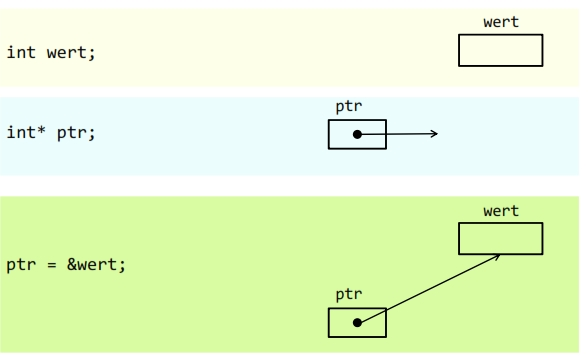
\includegraphics[width=1\textwidth]{pics/pointer_beispiel_1.jpg}
		\end{minipage}	
		%
		\begin{minipage}[t]{6 cm}
			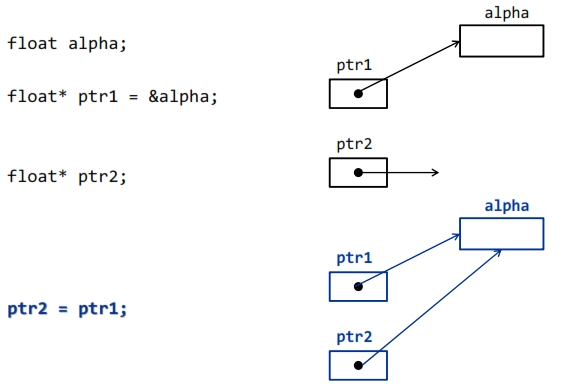
\includegraphics[width=1\textwidth]{pics/pointer_beispiel_2.jpg}
		\end{minipage}	
		%
		\begin{minipage}[t]{6 cm}
			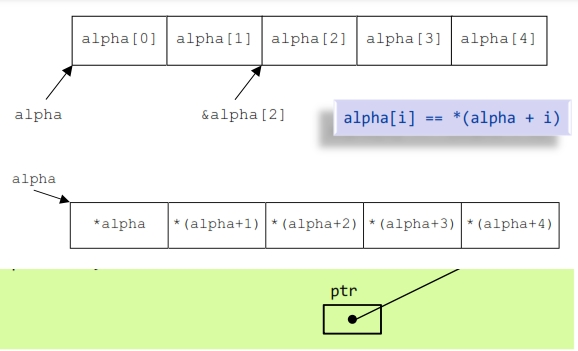
\includegraphics[width=1\textwidth]{pics/pointer_beispiel_3.jpg}
		\end{minipage}
		
	\subsubsection{Pointerarithmetik \verweis{10.1.1}}
		\begin{minipage}[t]{9 cm}
			\textbf{Zuweisung:} 
			\begin{compactitem}
				\item Pointer unterschiedlicher Datentypen dürfen einander nicht zugewiesen werden (Schutzmechanismus).
				\item Einem Pointer eines bestimmten Typs dürfen Pointer dieses Typs oder void-Pointer zugewiesen werden.
				\item Einem void-Pointer dürfen beliebige Pointer zugewiesen werden (nützlich aber gefährlich).
			\end{compactitem}
			\ \\
			\textbf{Vergleiche:} 
			\begin{compactitem}
				\item Bei Pointern desselben Typs funktionieren Vergleiche wie $==$, $!=$, $<$, $>$, $>=$, etc.
				\item Hintergrund: ein Pointer ist eine Adresse, d.h. die Vergleiche passieren mit den Adressen. Daraus ist klar, was die Vergleiche bewirken.
			\end{compactitem}
		\end{minipage}	
		\hspace*{0.5cm}
		\begin{minipage}[t]{9 cm}
			\textbf{Addition und Subtraktion:} 
				\begin{compactitem}
					\item Zu einem Pointer darf eine ganze Zahl oder ein anderer Pointer desselben Typs addiert werden.
					\item Von einem Pointer kann eine ganze Zahl oder ein anderer Pointer desselben	Typs subtrahiert werden.
					\item Wenn eine ganze Zahl n addiert / subtrahiert wird, so bewegt sich der Pointer	auf das nächste Element des Pointertyps. Die Zahl n wird also nicht als Byte interpretiert, der Pointer bewegt sich um $n*sizeof(Typ)$ Bytes.
				\end{compactitem}
				\ \\
				\textbf{Andere Operationen:} 
				\begin{compactitem}
					\item Andere Operationen sind nicht erlaubt!
				\end{compactitem}
		\end{minipage}	

	\subsection{Arrays \verweis{6.3}}
		Ein Array bietet eine kompakte Zusammenfassung von mehreren Variablen des gleichen Typs.
		
		\begin{minipage}[t]{10.5 cm}
			\subsubsection{Definition eines Arrays \verweis{6.3}}
				\vspace*{-0.3cm}\lstinputlisting[language=C,tabsize=2]{code/array_init.c}
				
			\subsubsection{Zeichenketten (Strings) \verweis{6.3}}
				\begin{compactitem}
					\item Ein String ist in C ein Array von Zeichen (char-Array).
					\item Ein String muss in C immer mit dem Nullzeichen $'\backslash0'$ \\
					abgeschlossen werden. Dieses benötigt eine Stelle im Array!					
				\end{compactitem}
				\lstinputlisting[language=C,tabsize=2]{code/array_string.c}
		\end{minipage}	
		%
		\begin{minipage}[t]{8.5 cm}
			\subsubsection{Zugriff auf ein Arrayelement \verweis{6.3}}
				Der Zugriff auf ein Element eines Arrays erfolgt über den Array-Index. Ist ein Array mit n Elementen definiert, so ist darauf zu achten, dass in C der Index mit 0 beginnt und mit n-1 endet.
				\lstinputlisting[language=C,tabsize=2]{code/array_zugriff.c}
		\end{minipage}	

		\begin{minipage}[t]{9 cm}
			\subsubsection{Äquivalenz von Array- und Pointernotation \verweis{10.1}}	
				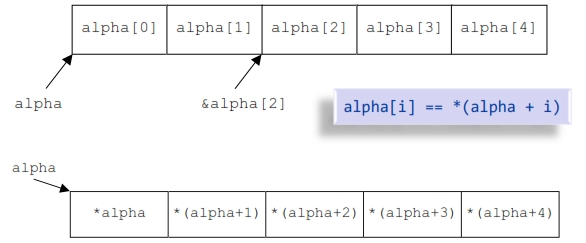
\includegraphics[width=1\textwidth]{pics/array_pointer.jpg}
				
			\subsubsection{Vergleichen von Arrays \verweis{10.1}}
			\begin{compactitem}
				\item In C gibt es keinen Operator $==$, der zwei Arrays miteinander vergleicht.
				\item Arrayvergleiche müssen explizit Element um Element durchgeführt werden oder der Inhalt der beiden Speicherbereiche wird mit Hilfe der Funktion	$memcmp()$ byteweise verglichen.
			\end{compactitem}
		\end{minipage}
		\hspace*{0.5cm}
		\begin{minipage}[t]{9 cm}	
			\subsubsection{Der Arrayname \verweis{10.1}}
				\begin{compactitem}
					\item Der Arrayname ist ein nicht modifizierbarer L-Wert.
					\item Der Arrayname ist ein konstanter Pointer auf das erste Element des Arrays und kann nicht verändert werden.
					\item Auf den Arraynamen können nur die beiden Operatoren $sizeof$ und $\&$ angewandt werden.
					\item Der Arrayname (z.B. $arr$ bei $int$ $arr[5]$), als auch der Adressoperator angewandt auf den Arraynamen ($\&arr$) ergeben einen konstanten Pointer auf das erste Element des Arrays, d.h. sie ergeben dieselbe Adresse. Der Datentyp ist allerdings unterschiedlich: \\
					Der Typ von $arr$ ist $int*$ \\
					Der Typ von $\&arr$ ist $int$ $(*)[5]$ (Pointer auf Array mit 5 int's)
					\item Einem Arraynamen kann kein Wert zugewiesen werden (einer Pointervariablen	schon).
				\end{compactitem}
		\end{minipage}
		
		\vspace*{0.1cm}
		
		\begin{minipage}[t]{9 cm}
			\subsubsection{Automatische Initialisierung \verweis{10.1.3}}	
				\begin{compactitem}
					\item Globale Arrays werden automatisch mit 0 initialisiert.
					\item Lokale Arrays werden nicht automatisch initialisiert.
				\end{compactitem}
				
			\subsubsection{Explizite Initialisierung \verweis{10.1.3}}	
				\begin{compactitem}
					\item Bei der Definition eines Arrays kann ein Array explizit ("manuell") initialisiert werden.
					\item Nach der Initialisierung können die Elemente nur noch einzeln geändert werden.
				\end{compactitem}
				\lstinputlisting[language=C,tabsize=2]{code/array_init_zuweisung.c}
				\begin{compactitem}
					\item Werden bei der Initialisierung weniger Werte angegeben als der Array Elemente hat, so werden die restlichen Elemente mit 0 belegt.
				\end{compactitem}
				\lstinputlisting[language=C,tabsize=2]{code/array_init_null.c}
				\begin{compactitem}
					\item Wird bei der Definition keine Arraygrösse angegeben, so zählt der Compiler die Anzahl Elemente automatisch (offenes Array oder Array ohne Längenangabe).
				\end{compactitem}
				\lstinputlisting[language=C,tabsize=2]{code/array_init_offen.c}
		\end{minipage}
		\hspace*{0.5cm}
		\begin{minipage}[t]{9 cm}	
			\subsubsection{Mehrdimensionale Arrays \verweis{10.1.4}}
				Das Array $int$ $alpha[3][4]$ kann folgendermassen aufgezeichnet werden: \\
				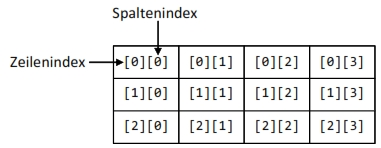
\includegraphics[width=1\textwidth]{pics/array_mehrdimensional.jpg}
			
			\subsubsection{Initialisierung eines mehrdimensionalen Arrays \verweis{10.1.4}}
				\lstinputlisting[language=C,tabsize=2]{code/array_init_mehrdimensional.c}
		\end{minipage}

		\subsubsection{Initialisierung von Zeichenketten \verweis{10.1.5 und Kapitel 10.1.6}}
			\lstinputlisting[language=C,tabsize=2]{code/string_init.c}
			
		\subsubsection{Übergabe von Arrays und Zeichenketten \verweis{10.2}}
			\begin{compactitem}
				\item Bei der Übergabe eines Arrays an eine Funktion wird als Argument der Arrayname übergeben (i.e. Pointer auf erstes Element des Arrays).
				\item Der formale Parameter für die Übergabe eines eindimensionalen Arrays kann ein offenes Array sein oder ein Pointer auf den Komponententyp des Arrays.
				\item Die Grösse des Arrays muss immer explizit mitgegeben werden.
				\item Zeichenketten sind char-Arrays und werden deshalb gemäss der oben erwähnten Punkte gehandhabt.
			\end{compactitem}
			\lstinputlisting[language=C,tabsize=2]{code/array_uebergabe.c}
			
		\subsubsection{Übergabe eines mehrdimensionalen Arrays}
			\lstinputlisting[language=C,tabsize=2]{code/array_uebergabe_mehrdimensional.c}